% !TEX root = thesis.tex
\chapter{考察と提言}
この章では、5章の結果に対する考察を行うと共に、考察結果を踏まえ、深層学習の実問題における効率的な応用方法について、提言を行う。

\section{全体のまとめ}
Pylearn2におけるMaxout Networkは、元論文に記されている精度こそ再現できなかったものの、MNISTの分類タスクにおいて最先端に近い精度を実現することが出来た。Maxout Networkを利用することで、少なくとも画像認識のタスクにおいて精度を向上させることが出来ると考えられる。\par
\section{分類誤差が大きくなってしまう原因の考察}
今回の実験では、MNISTの1次元版、2次元版共に、元の論文やPylearn2ソースコードの付属テキストに書いてあった分類誤差よりも、大きい誤差しか再現できなかった。また、この誤差が大きくなってしまう問題は、複数回の実験を行っても、解決しなかった。\par
分類精度が悪くなってしまった理由として、当初、図\ref{c6_maxout_cause}に挙げた3つの原因が考えられた。しかし、複数回実行しても全く同じ結果が出たため、乱数のシードを変更しない限り、内部的には全く同じ演算が成されていると考えられる。よって、「重みのランダム初期化」、つまり「ニューラルネットワークの接続の重みがランダムに決まっており、たまたま分類に不利な重みからスタートしたため、元の論文よりも悪い結果が出てしまった」という仮説は否定される。残る可能性は、「ソースコードのバージョン」と「ハードウェア構成の違い」であるが、GPUを始めとする各パーツの性能は、元論文の実験時に使われたものよりも、今回の実験で使ったものの方が高いため、「ハードウェアの性能」に原因を求めるのも難しい。残る可能性は「ソースコードのバージョン」である。これは、Pylearn2が依存しているライブラリの、NumpyやScipy、TheanoまたPylearn2自体などがアップデートされたことにより、内部的に細かい計算方法が変化し、分類誤差の再現性が下がってしまった、という仮説である。\par
実験の再現性については、Maxout Networkの元実験を行った方も、
\begin{quote}
All of Pylearn2's dependencies (Theano / Scipy / Numpy / etc.) make reproducibility
very difficult. As such, we are not currently going to make any effort to ensure that
all results are widely reproducible on a variety of platforms. Instead, we will
record the platform on which they were verified to be correct.
\end{quote}
と記している(Pylearn2のソースコード\footnote{\url{Pylearn2/scripts/papers/maxout/notes}}より引用)。彼らの認識でも、まずソースコードやライブラリのバージョンが重要であり、またハードウェアの性能も影響すると考えられていることが読み取れる。\par
\begin{figure}[tbp]
 \begin{center}
  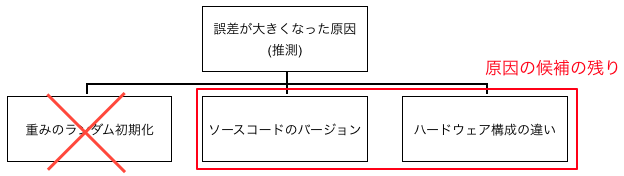
\includegraphics[width=80mm]{img/c6/maxout_error_cause}
 \end{center}
 \caption{Maxout NetworkによるMNIST分類実験で、誤差が論文より大きくなった原因}
 \label{c6_maxout_cause}
\end{figure}
\section{CIFAR10の実行時間が非常に長くなってしまう問題について}
今回の実験では、MaxoutによるCIFAR10の分類を、実行時間があまりにも長くかかるため、断念してしまった。実行時間をどうすれば短縮できるのか、特にハードウェアを変えず、分類精度も犠牲にしないで、出来れば長くとも1日程度の実行時間で収束させるための方法がないか、検討を重ねる必要がある。その後の実験により、モデルの学習中に統計情報を収集させる部分で時間がかかってしまっている可能性があるとわかっている。精度を変えずに時間短縮をするための、大きなポイントの1つとして、追求を続ける必要がある。\par
ハードウェアを買わず、既存のハードウェアをやりくりして性能を上げる方法として、複数台マシンによる分散処理が挙げられる。論文の中には、数日規模の計算を行っているものもあり、分散処理を行わせる価値は高い。例えば、\cite{krizhevsky2012imagenet}では、複数台のGPUマシンを用いて畳み込みネットワークの学習を行わせている。このとき、GPU間で計算結果を通信する部分がボトルネックになると予想されるが、この研究ではニューロンをGPUごとに分担させ、一部のレイヤーでのみ同期通信を行うことで、GPU間通信の回数を抑えて対処している。分散処理の弱点は通信自体にかかる時間だけではなく、同期部分において最も遅いマシンがボトルネックになってしまうという点もある。例えばGPUマシンとCPUマシンが混交している場合、CPUマシンの性能と同じ速度しか出なくなってしまうことが挙げられるが、この問題は、ある程度の回数まで同期の無視を認めることで解決できる\cite{ho2013more}。


\section{深層学習の利用法に関する提言}
Maxout Networkが良い精度を実現できたこと、改造のしやすさ、GPU利用の簡便さなどを考え合わせると、現時点では、Pylearn2を通して深層学習を利用するのが良いと考えられる。
深層学習を利用する上で、最も求められる高い識別性能は、Maxout Networkを利用することで担保できる。Maxout Networkは、画像に対しては畳み込みレイヤーと併用することにより、ほぼ最先端と遜色ない精度を実現することができる。また、対象が画像ではなく、1次元の広がりしかもたないデータの場合、畳み込みレイヤーを使うことは出来ないが、現時点では最も高い識別精度を出すことが出来る。この識別性能は、画像データだけでなく、他のデータを扱う際にも有用だと思われる。また、任意の連続関数を近似できるため、かつての単層パーセプトロンのように、理論的に学習できない関数が出現するということもない。深層学習に識別精度を求める場合、Maxout Networkを使うのが最も有効な方法の1つである。\par
Maxoutの既存実装としては、論文の著者自らが提供しているライブラリの、Pylearn2を使うのが最も確実である。この実装を使えば、論文にて述べられている分類精度にかなり近い精度を、実際に実現することができる。厳密には、論文の分類精度よりも、若干性能は劣化してしまうが、著者が実験を行ったときのハードウェアと、ソースコードのバージョンを揃えずとも、かなり近い精度を再現できることも、また事実であり、実用上はあまり問題にならないと考える。\par
深層学習の大きなネックの1つとして、その長い実行時間が挙げられる。この問題は、実行時にGPUを利用することによってかなり緩和できるが、CUDAを用いた専用のプログラムを書く必要があり、難易度が比較して高くなってしまう。この難点は、計算アルゴリズムを書くときに、数値計算/数式処理ライブラリであるTheanoを利用することで、かなり楽になる。Theanoで書いたプログラムは、GPU上でも利用でき、CPUのみのマシンでも、実行速度は下がるが問題なく動かすことができる。また、科学技術計算プログラムの記述においてメジャーなPythonで書かれており、C言語のプログラムに比べて記述が容易であるにも関わらず、事前にCUDAのコードを生成\&コンパイルする仕組みにより、C言語でCUDAのコードを全て記述した場合と代わらない速度で動かすことができる。\par
Pylearn2はTheanoの機能をフルに活用して記述されており、またSpaceクラスや画像による可視化など、Theanoに不足している部分にもフォローがされている。Pylearn2を使えば、Theanoの恩恵をそのまま受けることができる。この点でも、Pylearn2は望ましいと考えられる。\par
Pylearn2は、規模の比較的大きいライブラリではあるが、ソースコードは再利用性を強く意識して記述されており、モジュール化が明確である。LIBSVMのような、テキストファイルにデータを書くだけで利用できるような仕組みは残念ながら用意されていないが、例えば入力データを差し替えるだけならば、Datasetクラスの内容を把握して書くだけで済む。また、アルゴリズムにて使われているハイパーパラメータを調整するだけなら、ソースコードを書く必要すらなく、設定用のyamlファイルを変更するだけで調整を済ませることができる。この「利用する部分だけ把握すれば良い」という性質は、モジュール化の大きな利点であり、そのままPylearn2の大きな利点でもある。